% SKRIV GERNE KOMMENTARER UD FRA "USEPACKAGE" SÅ VI VED HVAD DE GØR :-)
\documentclass[a4paper]{article} 

\usepackage[utf8]{inputenc} % hedder den ikke utf8x? 
\usepackage[danish]{babel}

\usepackage[T1]{fontenc}

\usepackage{csquotes}
\usepackage{verbatim}

\documentclass[11pt]{article}

% You get CM (Computer Modern) if you don't use mathtime.  Don't use
% times because then the math will be in CM and the text will be in
% Times; the result looks pretty bad.  The [mtbold] option makes it
% so that boldface font looks correct in math mode.  And you'll need
% it if you need to use the latexsym package.  (The clrscode package,
% which we'll see later in the course, requires latexsym, so if you're
% going to use mathtime and clrscode, you'll need to give the [mtbold]
% option to mathtime.)

% Tell LaTeX that we are using ISO-8859-1 encoding for input files
\usepackage[utf8]{inputenc} % danish characters on PC + MAC + Linux

\usepackage{times}
\usepackage{clrscode3e}
\newcommand\tabs[1]{\hspace*{#1pt}}     %% tabspaces in pt


\usepackage[margin=2.5cm]{geometry}

\usepackage{hyperref}
\usepackage{soul} % strikeout a line (eg. \st{Hellow world})


\usepackage{graphicx} % Images
\graphicspath{ {./images/} }

\usepackage{listings}
\usepackage[table,xcdraw]{xcolor}
\usepackage{color}

\definecolor{bluekeywords}{rgb}{0.13,0.13,1}
\definecolor{greencomments}{rgb}{0,0.5,0}
\definecolor{turqusnumbers}{rgb}{0.17,0.57,0.69}
\definecolor{redstrings}{rgb}{0.5,0,0}

\usepackage{amsmath}

\title{Diskret Matematik og Algoritmer
\\Ugeopgave 4g}
\author{Mads Pontoppidan Haderup (xjr983), Ken Kjøller Andersen (zcj256)\\
og Christian Handest (lzp959)}

\begin{document}
\maketitle % Insert title etc.

%%%%%%%%%%%%%%%%%%%%%%%%%%%%%%%% DEL 1 %%%%%%%%%%%%%%%%%%%%%%%%%%%%%%%%


\pagebreak
\section{DEL 1}
Lad S være en sorteret liste af tal repræsenteret ved hjælp af en dobbelthægtet liste (eng. double linked list). Målet med denne delopgave er at vedligeholde S når nye tal indsættes i S, således at S fortsat er sorteret.

\subsection{DEL 1A}
\begin{enumerate}
\item Beskriv hvilke felter (eng. attributter) en knude (eng. object/node) i listen S skal indeholde. 

Et knudeobjekt har 3 felter: Key, next og prev. Key er et heltal, next
og prev er pegere som peger på henholdsvist næste og forrige objekt i S.

\item Lav pseudokode der givet et heltal z, opretter en liste med dette ene tal.
\end{enumerate}

\begin{figure}[h]
\centering
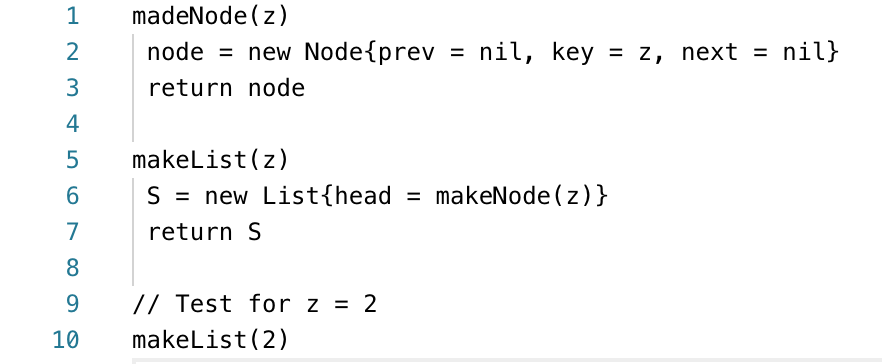
\includegraphics[width=8cm]{del1ab.png}
\end{figure}


\subsection{DEL 1B}
Lav pseudokode F(S,z), der tager en sorteret liste S, og et heltal z. Funktionen skal indsætte heltallet i S, sådan at S stadig er sorteret. Det skal ske på følgende måde: F gennemløber S fra starten indtil den finder det rigtige sted at indsætte heltallet z. Herefter indsættes z.

\begin{figure}[h]
\centering
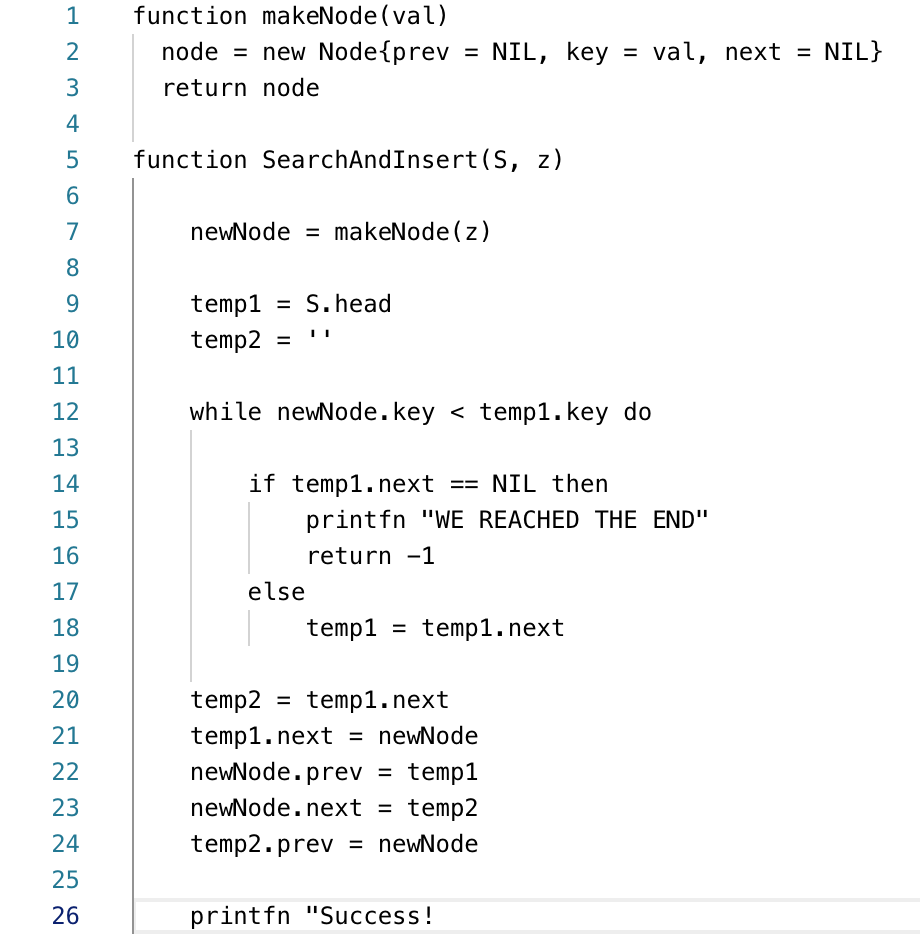
\includegraphics[width=8cm]{del1b.png}
\end{figure}


\subsection{DEL 1C}
Argumentér for at din funktion i værste fald bruger $\Theta(n)$ tid på indsættelse af et enkelt element, hvor n er antallet af tal i listen.

\bigskip\noindent
Funktionen har et while loop, som først stopper når det har fundet den korrekte placering for z i den sorterede liste S. Sagt med andre ord foregår der en lineær søgning, hvor while loopet ved med at iterere over nodernes keys, indtil z er større end den fundne key. I værste fald vil z skulle placeres bagerst i listen, hvilket svarer til O(n). Men da z i alle andre tilfælde placeres forrest eller inde i listen, vil den gennemsnitlige placering blive betragtet i $\Theta(n)$ tid. 

\subsection{DEL 1D}
Lad listen S være tom til at starte med. Der indsættes herefter n heltal. Et af gangen. Når det sidste heltal er indsat vil S være en sorteret liste bestående af de n indsatte tal. Argumentér for at vi på denne måde har sorteret n tal i O(n2) tid.

\noindent
I ovenstående funktion insertAtEnd(n) indgår både et for- og nested while loop. Begge loops har en køretid på O(n) tid. Af den årsag vil funktionens samlede køretid blive O(n*n) = $O(n^2)$

\subsection{DEL 1E}
Hvilken sorteringsalgortime svarer forrige delopgave til?

\bigskip\noindent
Forrige algoritme svarer til insertion-sort. Da forrige algoritme
sorterer som man ville sortere kort man får på hånden. ligeledes
sorterer insertion sort. Dvs. man tager et kort, ser tallet, og
sætter kortet ind på den plads, hvor tallet er højere end de forrige.

\section{DEL 2}
Lad S være en sorteret liste af n heltal som i ovenstående Del 1.

\subsection{DEL 2A}
Lad $n = k * k$ være således at $k = \sqrt{n}$ er et heltal. Listen S kan opdeles i k mindre sorterede lister, $l_1, l_2$ ... $l_k$, hvor hver af de k små lister, består af k elementer. Lav en dobbelthægtet liste B. Knuderne i listen B indeholder ikke tal som S, men pegere pa (ud over next/prev). Det i’te elements peger pa skal pege på listen li. Beskriv hvorledes S kan opdeles og B oprettes. Angiv ligeledes køretiden for dette.

En måde at gøre det på er at iterere over listen S for at finde n så kvadratroden af n kan findes. Hvis n er kendt i forvejen kan vi nøjes der med at finde kvadratroden af n. Herefter skal  der oprettes en ny dobbelthægtet liste til at hvis første elements pa peger på det første element i listen S. Herefter kan der med en løkke der tager k skridt i S per iteration og tilføjer et element til B så elementets pa peger på elementer i listen S. 


\subsection{DEL 2B}
Hvor lang tid, angivet i O-notation, tager det at gennemløbe listen B, hvis S indeholder n elementer?

Da køretiden for at gennemløbe listen S er O = (n), vil køretiden for at gennemløbe listen B som kun indeholder k elementer være O = (\sqrt{n})


\subsection{DEL 2C}
Lav en funktion G der er givet S og B og et nyt heltal x. S indeholder $n = k * k$ elementer og B indeholder k elementer, som beskrevet ovenfor. G skal indsætte x i S ved at bruge B. Din funktion skal bruge tid $O(n\sqrt{n})$.

\begin{codebox}
\Procname{$\proc{Insert-Sorted-List}(S, B, x)$}
\li $b \gets B.nil.next$  
\li \While $b.pa \neq B.nil$ \And $b.pa \neq x$ \And $b.pa < x$  
\li \Do
$\id{b.pa} \gets b.next$
\li \Comment Insert $A[j]$ into the sorted sequence
\End
\li $i \gets b.pa$
\li \While $i \neq S.nil$ \And $i.key \le x$
\li \Do
$i \gets i.next$ 
\End
\li $x.next \gets S.i.next$
\li $S.i.next \cdot prev \gets x$
\li $S.i.next \gets x$
\li $x.prev \gets S.i$
\End
\end{codebox}

\subsection{DEL 2D}
(frivillig – man behøves ikke at lave denne opgave) Vis at ovenstående tankegang kan bruges til at sortere n tal i $O(n\sqrt{n})$ tid.

\end{document}
